\section{Component Diagram}
\label{sec:implementation:component-diagram}

\Cref{fig:implementation:component-diagram:wear} shows a component diagram of the primary components involved in the application developed for the Android Wear smartwatch. The component diagram illustrates which key components are involved in the software and how they interact with each other.
The diagram focus on the smartwatch as most of our development was concentrated on that platform.

Below is a brief description of the components in the diagram. Notice the note in the diagram. Components which communicate without an \emph{assembly connector}, i.e. communicating using a required and a provided interface, communicate without the use of Java interfaces, \eg~invocation of public methods that are not part of a Java interface. Since the components are still considered to be independent of each other, it makes sense to revisit the implementation to communicate using assembly connectors, i.e. Java interfaces. When information is passed without the use of assembly connectors, the edge is annotated with the information being passed between the components.

\begin{description}
\item[PositionManager] Responsible for determing which room the user is in.
\item[PositionContextualInformationProvider] Provides the context recognizer with information about the users position. The provider encapsulates the Room and Room\_Action nodes of the Bayesian network and computes evidence for all rooms.
\item[GestureContextualInformationProvider] Provides the context recognizer with information about the gesture the user performed. The  provider encapsulates the Gesture and Gesture\_Action nodes of the Bayesian network and computes evidence for all gestures.
\item[ContextRecognizer] Determines an appropriate action to trigger based on the information provided by \texttt{PositionContextualInformationProvider} and \texttt{GestureContextualInformationProvider}.
\item[GestureRecognizer] Given X, Y and Z-accelerations obtained from the accelerometer of the smartwatch, the component scores the gesture templates and thus determines the gestures the user is likely to have made.
\item[OpenHABClient] Communicates with openHAP over HTTP.
\item[App UI] The component represents the UI of the Android Wear smartwatch application.
\end{description}

For a more detailed description of the components involved in the context engine,  refer to \Cref{sec:implementation:context-engine}.

\begin{figure}[h!]
\centering
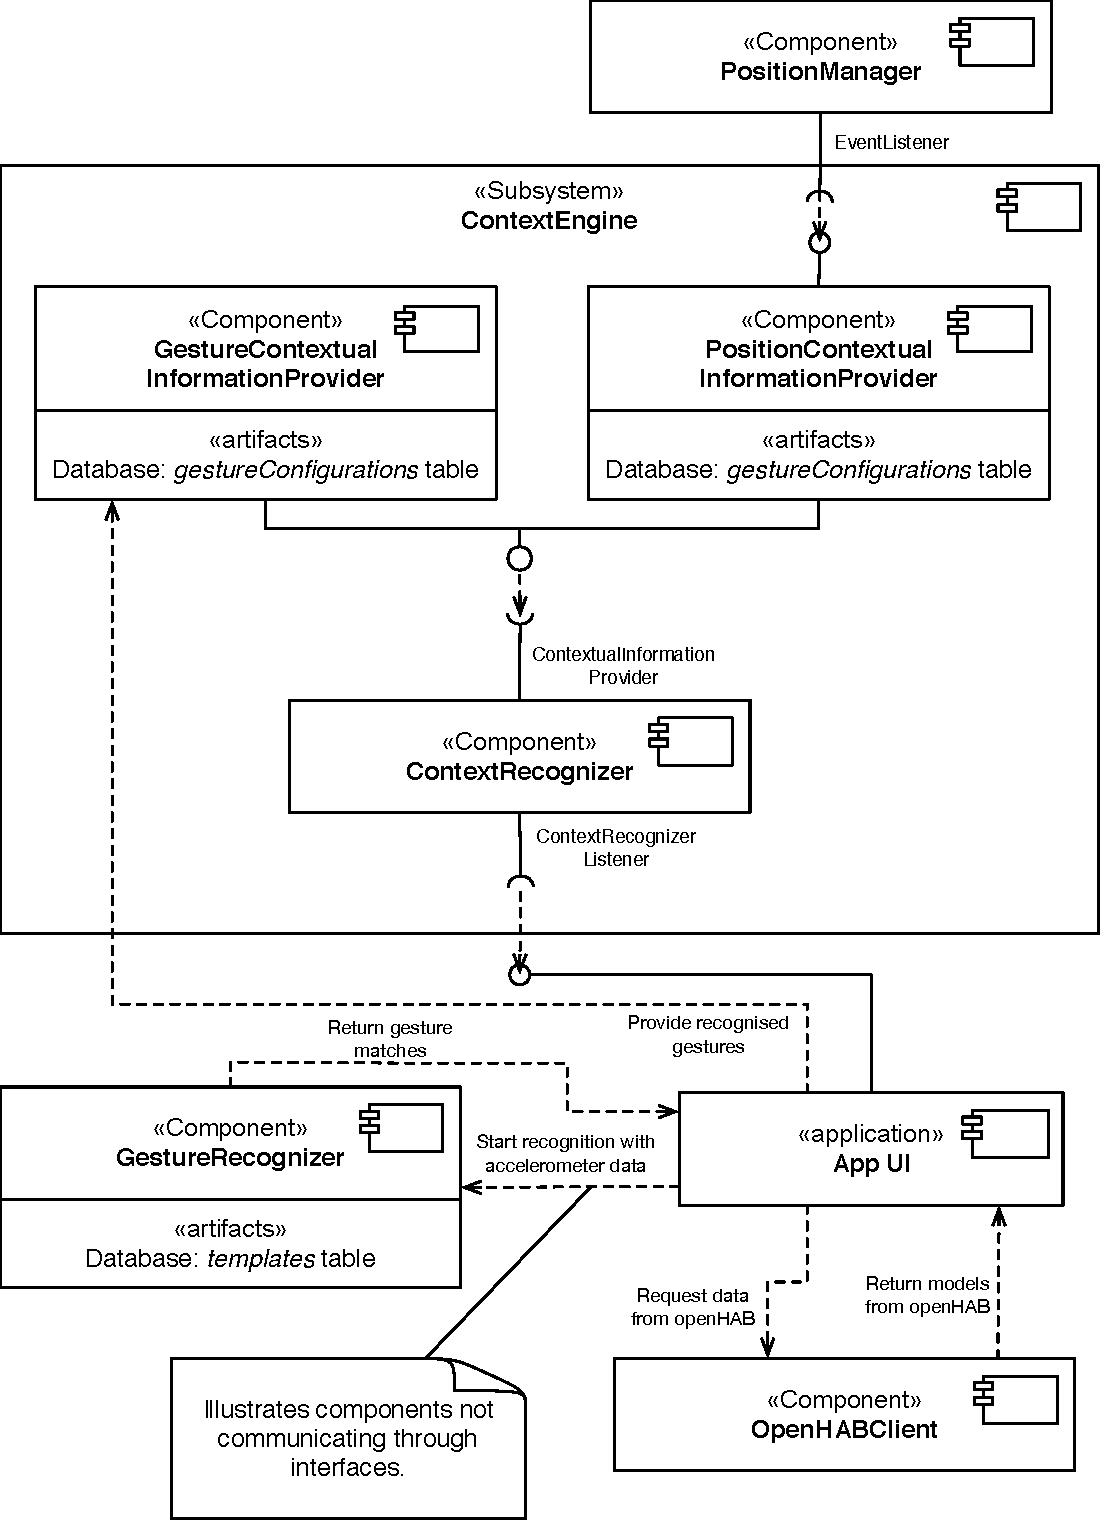
\includegraphics[width=\textwidth]{images/component-diagram-wear}
\caption{Component diagram showing the primary components of the Android Wear application.}
\label{fig:implementation:component-diagram:wear}
\end{figure}

%%% Local Variables:
%%% mode: latex
%%% TeX-master: "../../master"
%%% End:
